% Matlab 的程序调试及其他功能
% Matlab|调试|调试器|breakpoing

\pentry{Matlab 的函数\upref{MatFun}}

\subsection{程序调试}
\begin{figure}[ht]
\centering
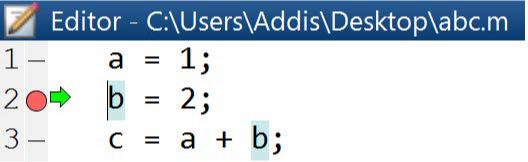
\includegraphics[width= 6cm]{./figures/MatOtr1.png}
\caption{在行首设置 Breakpoint}\label{MatOtr_fig1}
\end{figure}

若要调试程序,可选择一行代码并单击该行前面的横线,这时会出现红色圆点 Breakpoint (\autoref{MatOtr_fig1}),程序运行到 Breakpoint 会暂停.

此时要查看变量情况,可通过 Workspace 查看各个变量的情况,也可用光标悬停在某个变量上.还可以用 Command Window 改变某些变量的值,或画图等.在这种调试状态下,也可以通过 Edit 菜单中的一些按钮控制接下来程序如何运行(\autoref{MatOtr_fig2}).
\begin{figure}[ht]
\centering
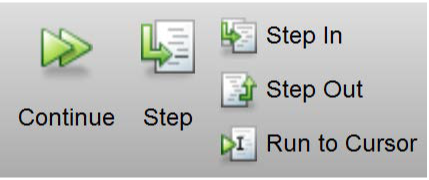
\includegraphics[width= 5cm]{./figures/MatOtr2.png}
\caption{Step 菜单}\label{MatOtr_fig2}
\end{figure}
其中“Continue”(快捷键 F5)是继续运行直到下一个 Breakpoint 或结束.“Step”(F10)是运行到下一行,“Step In”(F11)是进入子程序并暂停,“Step Out”是运行完当前子程序并回到子程序被调用的地方.“Run to Cursor”是运行到光标所在处.

\subsection{\x{warning} 和 \x{error} 函数}
有时候当我们的程序中出现了某个错误时, 程序会终止并在控制行中返回一个错误信息, 例如我们给 \x{sin} 函数输入两个变量时, 控制行的 \x{error} 信息将提示变量个数太多.
\begin{lstlisting}[language=MatlabCom]
>> sin(1,2)
Error using sin
Too many input arguments.
\end{lstlisting}
另一些情况下当错误不是那么严重时, 我们会得到一个 \x{warning} 提示, 程序在输出提示后将继续运行.

我们可以在我们自己的脚本或函数中用 \x{error} 或 \x{warning} 函数达到同样的效果

\code{MatOtr}

当 \x{error} 或 \x{warning} 函数被执行时, 控制行不但会输出对应的字符串, 还会输出它们所在的文件和行号, 如
\begin{lstlisting}[language=MatlabCom]
>> myfun w
Warning: this is a warning
> In myfun (line 3)
\end{lstlisting}
单击 \x{myfun} 或 \x{line 3}, 可在 Editor 中显示对应位置. 若 \x{myfun} 函数被其他函数调用, 那么调用的位置也会被逐级列出. 使用 \x{warning} 的效果类似, 但程序不会被终止.

\subsection{分节}
在行首用两个百分号“\x{\%\%}” 可以对代码进行分节(\autoref{MatOtr_fig3}).这样做一是可以使代码结构更清晰,二是可以单独选择某一节运行(Edit 菜单中的“Run Section”按钮).
\begin{figure}[ht]
\centering
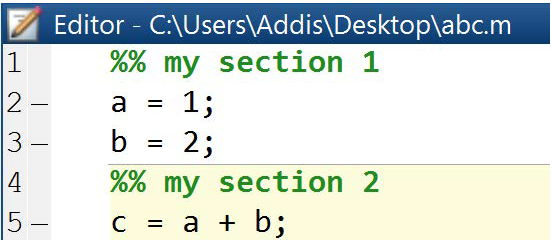
\includegraphics[width= 6cm]{./figures/MatOtr3.png}
\caption{代码分节}\label{MatOtr_fig3}
\end{figure}

\subsection{工具箱(Toolbox)}
在购买和安装 Matlab 软件时,可以选择各种各样的工具箱,常用的工具箱有曲线拟合(Curve Fitting,从离散的数据点得到一条曲线),图像处理(Image Processing,图像变换,增强,降噪,二值化等),图像获取(Image Acquisition,从相机获取图像),Matlab 编译器(MATLAB Compiler,编译代码,提高运行速度).注意使用了工具箱功能的代码在没有工具箱的 Matlab 软件上将无法运行.




